\documentclass{article}
\usepackage{amsmath}
\usepackage{amssymb}
\usepackage{amsfonts}
\usepackage{dsfont}
\usepackage{graphicx} % Required for inserting images
\usepackage{listings}
	\lstset{language=R,
    basicstyle=\small\ttfamily,
    stringstyle=\color{green},
    otherkeywords={0,1,2,3,4,5,6,7,8,9},
    morekeywords={TRUE,FALSE},
    deletekeywords={data,frame,length,as,character},
    keywordstyle=\color{blue},
    commentstyle=\color{green},
}
\usepackage{xcolor}
\usepackage{array}
\usepackage[vmargin=2cm,hmargin=2cm]{geometry}


\title{TP2-ADM}
\author{Guillaume Bernard-Reymond et Lorenzo Gaggini}
\date{Décembre 2023}

\begin{document}
\newcommand{\norme}[1]{\left\| #1\right\|}
\newcommand{\tr}{\text{tr}}
\maketitle
\setlength{\parindent}{0pt}

Dans ce TP, nous avons à notre disposition un jeu données concernant 100 villes françaises dont on connaît 54 indicateurs répartis en quatre grands thèmes : Economie, Risques, Nature et Culture.\\

Nous avons décidé d'utiliser la bibliothèque Factoshiny pour son confort d'utilisation. 

\section{ACP normé sur l'ensemble des variables}

\subsection{Etude de la variance cumulée}

Dans un premier temps, nous nous intéressons à la variance cumulée et notamment les grands décrochements. Nous allons devoir faire un choix qui ne sera malheureusement pas sans perte d'informations.

Voici le graphique des valeurs des valeurs propres : 

\centerline{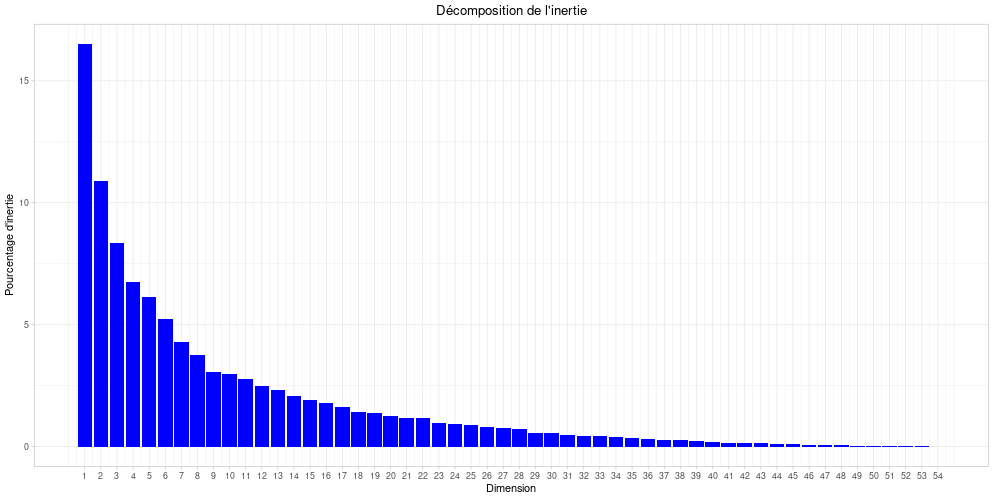
\includegraphics[width=\linewidth]{images/ACP_vp}} 

Voici le tableau des variances cumulées :

\begin{center}
 \begin{tabular}{|l|*{8}{>{\centering\arraybackslash}p{1cm}|}}
 \hline 
 \rule[-1ex]{0pt}{2.5ex} Valeurs propres & Dim.1  & Dim.2 &  Dim.3 &  Dim.4 &  Dim.5 &  Dim.6 &  Dim.7 & Dim.8\\ 
 \hline 
 \rule[-1ex]{0pt}{2.5ex}  Variance & 8.914 &  5.889  & 4.511 &  3.646  & 3.306 &  2.820  & 2.326 & 2.041\\
 \hline 
 \rule[-1ex]{0pt}{2.5ex} 
$\%$ of var. &  16.508 & 10.906 &  8.353 &  6.752  & 6.121 &  5.222 &  4.307 & 3.780 \\
 \hline 
 \rule[-1ex]{0pt}{2.5ex} 
Cumulative $\%$ of var. & 16.508 & 27.414 & 35.767 & 42.519 & 48.641 &  53.862 & 58.169 & 61.949 \\
\hline
\end{tabular}
\end{center}

Le nombre d'axes choisis pour mener l'étude de l'ACP est le même pour les individus que les variables car les valeurs propres des opérateurs d'inertie directe et duale sont les mêmes à un certain nombre de valeur propres nulles près. Ainsi dans toute la suite du rapport, nous ne distinguerons plus, sauf mention explicite du contraire, la variance cumulée des individus et celle des variables.\\

On peut observer un décrochement après la troisième valeur propre.  Nous nous contenterons des trois premiers axes avec une inertie cumulée de seulement 35.767\%. Pour être plus exhaustif, on pourrait prendre davantage de valeurs propres. Toutefois, ne pouvant observer de véritables décrochements dans les valeurs propres, nous serions obligés d'en garder environ 8 car la différence entre deux valeurs successives est faible. Le temps de traitement en deviendrait trop long.  

\subsection{Etude des variables}

Sur les graphiques suivants sont marqués les 10 variables les plus contributives à la fabrication des axes : 

\begin{center}
\begin{tabular}{ccc}
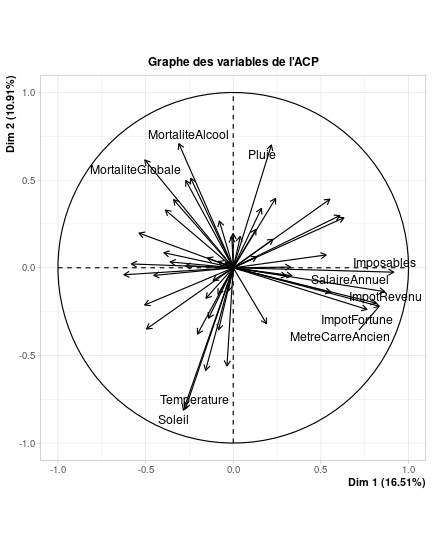
\includegraphics[width=0.3\linewidth]{images/ACP_var_12_contrib.png} & 
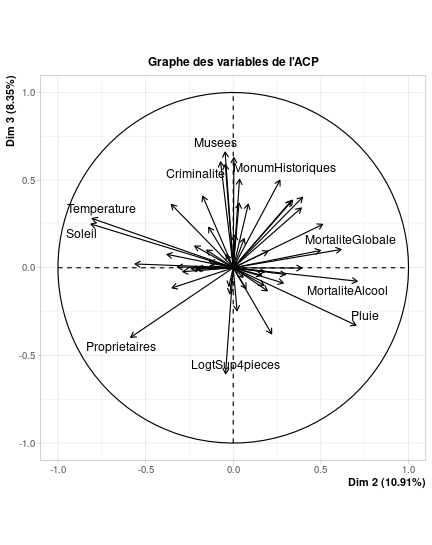
\includegraphics[width=0.3\linewidth]{images/ACP_var_23_contrib.png} & 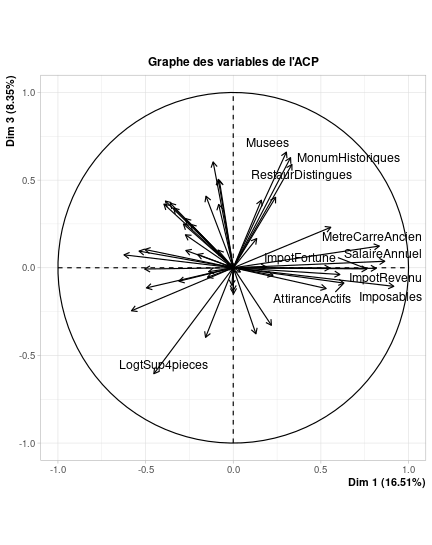
\includegraphics[width=0.3\linewidth]{images/ACP_var_13_contrib.png}• \\ 
\end{tabular} 
\end{center}

{\large \textbf{Axe 1}}

\begin{itemize}
	\item[$\bullet$] \textbf{Contribution}

	Tout d'abord, observons que $ \frac{1}{54}\approx 2\%$ ce qui nous 	pousse à ne considérer que les variables dont la contribution est très supérieure à $2\%$. On trouve alors : \emph{Imposables} (9,41\%), \emph{SalairesAnnuels} (8,38\%), \emph{MetreCarreAncien} (7,75\%), \emph{ImpotRevenu} (7,46\%) et \emph{ImpotFortune} (6,52\%). En additionnant, leur contribution on obtient : $39,52\%$ ce qui est très supérieur à $5\times 2\%=10\%$. Ce sont donc des variables économiques qui contribuent en une part importante à la fabrication de l'axe 1. On voit d'ailleurs sur le plan (1,2), ce groupe de variables allant dans la même direction.

	\item[$\bullet$] \textbf{Originalité : COS2}
	
	On retrouve ici, les mêmes variables que précédemment et dont l'originalité est principalement décrite par l'axe 1 : \emph{Imposables} (0,84), \emph{SalairesAnnuels} (0,75), \emph{ImpotFortune} (0,66), \emph{MetreCarreAncien} (0,65). \\
	
On peut en conclure que cet axe 1 décrit des marqueurs de richesse.
	
\end{itemize}

\bigskip

{\large \textbf{Axe 2}}

\begin{itemize}
\item[$\bullet$] \textbf{Contribution}
Parmi les variables dont la contribution est très supérieure à $2\%$, il y a : \emph{Soleil} (11,20\%), \emph{Température} (11,01\%), \emph{MortaliteAlcool} (8,50\%), \emph{Pluie} (8,33\%) et \emph{MortaliteGlobale} (6,43\%). De manière cumulée, on obtient 45,47\%. Sur la représentation du plan (1,2), on voit ces variables s'opposer : \emph{Soleil} et \emph{Température} d'un côté, les trois restantes de l'autre.  

\item[$\bullet$] \textbf{Originalité : COS2}
L'originalité des variables \emph{Soleil} et \emph{Temperature} est capturée à hauteur de $0,66$ et $0,65$ par l'axe 2. Si on leur ajoute leurs valeurs sur les axes 1 et 3, on trouve \emph{Soleil} : 0,8 et \emph{Temperature} : 0,8 aussi. Pour la \emph{MortaliteAlcool}, on a $0,50$ sur l'axe 2 et $0,61$ si l'on considère les trois axes. De même, le COS2 de la mortalité globale est de $0,38$ le long de l'axe 2 et $0,64$ si l'on considère les 3 axes. Enfin pour la pluie, on trouve $0,49$ sur l'axe 2 et $0,65$ pour les 3 axes.

Ici on commence à avoir une idée de ce que semble représenter cet axe : une opposition entre le Nord et le Sud de la  France. L'étude ultérieure des individus nous permettra d'en dire  certainement plus.

\end{itemize} 

\bigskip

{\large \textbf{Axe 3}}

\begin{itemize}
\item[$\bullet$] \textbf{Contribution}

Voici un tableau des variables les plus contributives à la fabrication de l'axe 3 : 

\begin{tabular}{|l|c|c|c|c|c|c|}
\hline 
Variables & Musées  & MonumentHistorique & LogtSup4Pieces & Criminalite & RestauDistingues & Total \\ 
\hline 
Contribution & 9,65 & 8,15 & 8,10 & 8,08 & 7,70 & 41,68 \\ 
\hline 
\end{tabular} 

\item[$\bullet$] \textbf{Originalité : COS2}

Pour ce qui est de l'originalité, on ne retrouve rien de très significatif. Celle-ci semble être diluée dans davantage d'axes que les 3 considérés. 

\begin{tabular}{|l|c|c|c|c|c|}
\hline 
Variables & Musées  & MonumentHistorique & LogtSup4Pieces & Criminalite & RestauDistingues \\ 
\hline 
Originalité sur l'axe 3 & 0,44 & 0,39 & 0,37 & 0,36 & 0,35  \\ 
\hline
Originalité sur les 3 axes & 0,53 & 0,5 & 0,58 & 0,38 & 0,46  \\ 
\hline  
\end{tabular} 

Si l'on observe les plans (2,3) et (1,3), on peut voir un faisceau entre des variables culturelles \emph{Musées}, \emph{MonumentHistorique} et \emph{RestauDistingues}, la variable \emph{LogtSup4Pieces} étant elle négativement corrélée aux trois précédentes. L'originalité de la variable criminalité n'étant finalement pas suffisamment décrite par l'axe 3, on peut supposer que l'axe 3 reflète plutôt une tendance culturelle et qui va opposer grandes et petites villes. 
\end{itemize}

\subsection{Etude des individus}

Voici le graphique du plan (1,2) avec les 10 individus les plus contributifs : 

\centerline{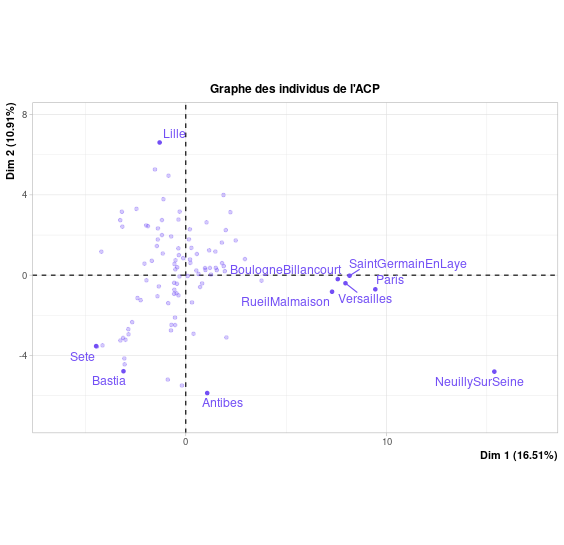
\includegraphics[width=0.5\linewidth]{images/ACP_ind_12_contrib}} 

Pour ce qui concerne la contribution, nous comparerons les valeurs avec la contribution moyenne $\frac{1}{100}=0,01$.

\bigskip

{\large \textbf{Axe 1}}

\begin{itemize}
\item[$\bullet$] \textbf{Contribution} 
Six villes ont une contribution forte pour l'axe 1 dont une plus particulièrement : 

\begin{center}
\begin{tabular}{|l|*{7}{m{1.7cm}|}}
\hline 
Individus & Neuilly-Sur-Seine  & Paris & Saint-Germain-en-Layes & Versailles & Boulogne-Billancourt & Rueil-Malmaison & Total \\ 
\hline 
Contribution & 26,51 & 10,0 & 7,46 & 7,10 & 6,43 &  5,96 & 63,46 \\ 
\hline 
\end{tabular}
\end{center}

La contribution de ces six villes est très largement supérieure à la contribution moyenne de $6\%$.

\item[$\bullet$] \textbf{Originalité : COS2}

Les villes dont l'originalité est largement supportée par l'axe 1 sont les mêmes que précédemment à l'exception notable de Paris : 

\begin{center}
\begin{tabular}{|l|*{6}{m{2cm}|}}
\hline 
Individus & Versailles  & Saint-Germain-en-Layes & Neuilly-Sur-Seine  & Boulogne-Billancourt &  Rueil-Malmaison \\ 
\hline 
Originalité & 0,73 & 0,67 & 0,65 & 0,61 & 0,57\\ 
\hline 
\end{tabular}
\end{center} 

L'originalité de Paris le long de cet axe est seulement de 0,25. Ceci semble indiqué que Paris n'est pas seulement originale par sa dimension économique mais que son originalité est multiple. 
\end{itemize}

Ce que l'on peut conclure de cette étude de l'axe 1, c'est que ce dernier représente effectivement des variables économiques et que quelques villes de l'Ouest parisien contribue fortement à son orientation. Si l'on met côte à côte la plan (1,2) du graphe de l'ACP des variables et celui des individus, on remarque évidemment une direction similaire entre les variables étudiées et les villes contributives.

\bigskip

{\large \textbf{Axe 2}}

\begin{itemize}
\item[$\bullet$] \textbf{Contribution}

Les principales contributions à la construction de l'axe 2 sont données par 6 villes : \emph{Lille} (7,42\%), \emph{Antibes} (5,85\%), \emph{Cannes} (5,13\%), \emph{Valenciennes} (4,71\%), Nice (4,60\%) et Saint-Denis (4,17\%). En additionnant leur contribution, on obtient 31,88\%. 

\item[$\bullet$] \textbf{Originalité : COS2}

Les cnq villes dont l'originalité est décrite partiellement par cet axe 2 sont : \emph{Lille} (0,47), \emph{Antibes} (0,44), \emph{Troyes} (0,42), \emph{Nice} (0,40) et \emph{Valenciennes} (0,38).
\end{itemize}

De cet axe 2 se dégage un axe Nord-Sud. Au Nord, des villes pluvieuses avec une mortalité globale supérieure et au Sud des villes chaudes et ensoleillées.

L'édition du plan (2,3) nous montre un regroupement de villes du Sud :

\centerline{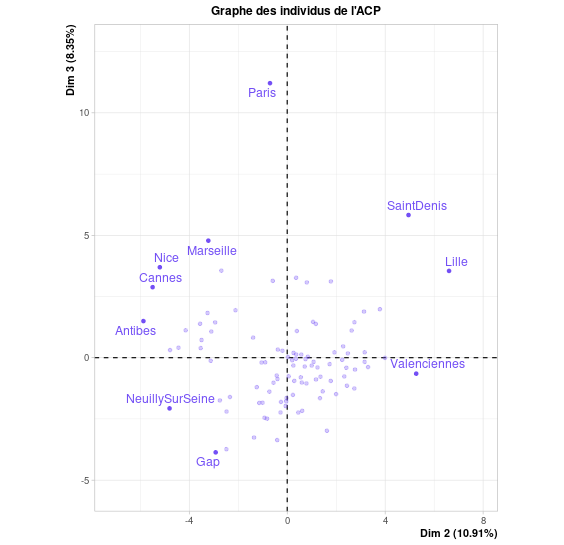
\includegraphics[width=0.5\linewidth]{images/ACP_ind_23_contrib}} 

Ce regroupement se trouve être justement dans la même direction que celui des variables \emph{Soleil} et \emph{Temperatures}.

\bigskip

{\large \textbf{Axe 3}}

Voici le plan (1,3) des individus : 

\centerline{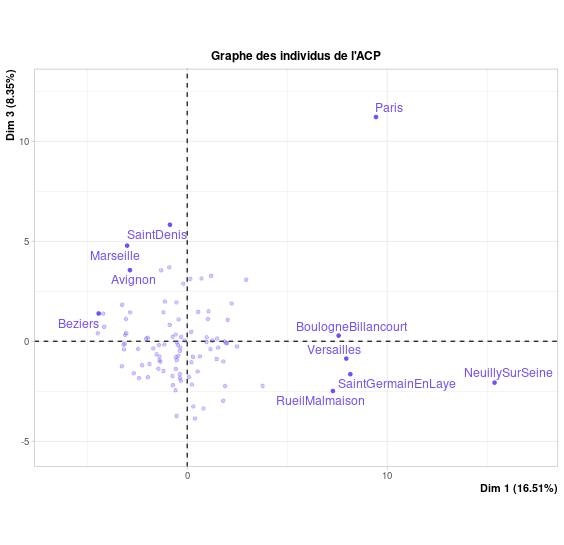
\includegraphics[width=0.5\linewidth]{images/ACP_ind_13_contrib}} 

\begin{itemize}
\item[$\bullet$] \textbf{Contribution}

On trouve ici quelques contributeurs importants et notamment une ville singulière \emph{Paris} contribuant à hauteur de $27,86\%$. Les deux autres villes sont \emph{Saint-Denis} (7,53\%) et Marseille (5,06\%). Dans une moindre mesure : \emph{Gap} (3,31\%) et \emph{Cholet} (3,09\%) contribue à la construction de cet axe.

\item[$\bullet$] \textbf{Originalité COS2}

Aucune ville ne semble être majoritairement décrite par cet axe 3. Toutefois on peut remarquer un fait notable. Nous avions dit que Paris, bien que contributeur de l'axe 1, ne voyait pas son originalité y être décrite. Paris se trouve être plus original selon cet axe 3 (0,35) auquel il participe grandement à sa construction. Les villes contributrices tirent une part de leur originalité de cet axe : \emph{Marseille} (0,29),  \emph{Cholet} (0,28) \emph{Saint-Denis} (0,26) et Gap (0,22).

Enfin \emph{La-Roche-Sur-Yon} a un COS2 égale à 0,31.
\end{itemize}

En superposant les plans où se trouvent l'axe 3, on remarque évidemment que les variables contributives à sa construction la position de Paris ne sont pas étrangères. La direction et la même et cela est du au fait que Paris a une contribution majeure à cet axe. Elle en tire d'ailleurs son originalité principale. Cet axe semble être celui des marqueurs culturels. 

\subsection{Conclusion}

On retrouve dans cet ACP, les résultats obtenus dans le TP2 où le dendogramme donnait une impression visuelle de former 3 classes : 

\centerline{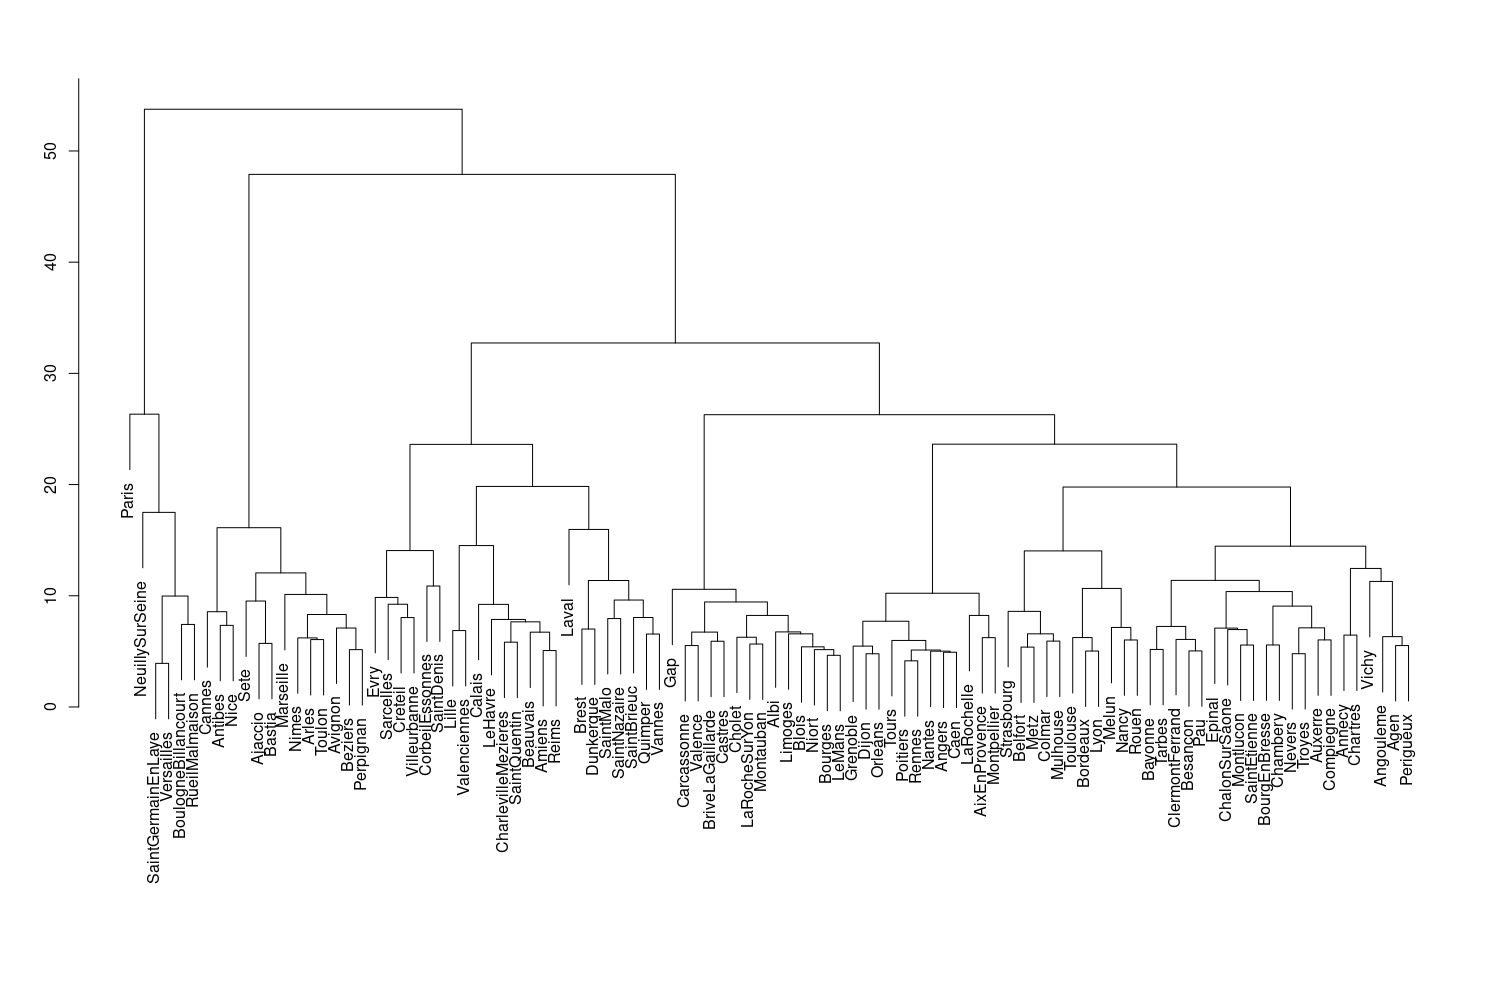
\includegraphics[width=0.5\linewidth]{images/Dendo}} 

On retrouve dans cette ACP, 3 axes principaux : 
\begin{itemize}
\item[$\bullet$] \textbf{Axe 1 :} axe à dominante économique avec de gros contributeurs se caractérisant par une position géographique bien particulière : l'Ouest parisien. 
\item[$\bullet$]  \textbf{Axe 2 :} celui-ci oppose le Sud ensoleillé et chaud au Nord pluvieux dont certaines variables au caractère plus morbide sont contributrices. 
\item[$\bullet$] \textbf{Axe 3 :} Cette fois ci c'est la culture qui se distingue mais la culture parisienne. En effet, il s'agit d'un contributeur majeur isolé à sa fabrication.  
\end{itemize}

\section{ACP de rang sur l'ensemble des variables}

Après avoir obtenu la matrice des rangs, nous lançons l'ACP avec Factoshiny. 

	\subsection{Etude de la variance cumulée}
	
Nous nous intéressons, comme pour l'ACP normée, aux valeurs propres dont voici le graphique :
	
\centerline{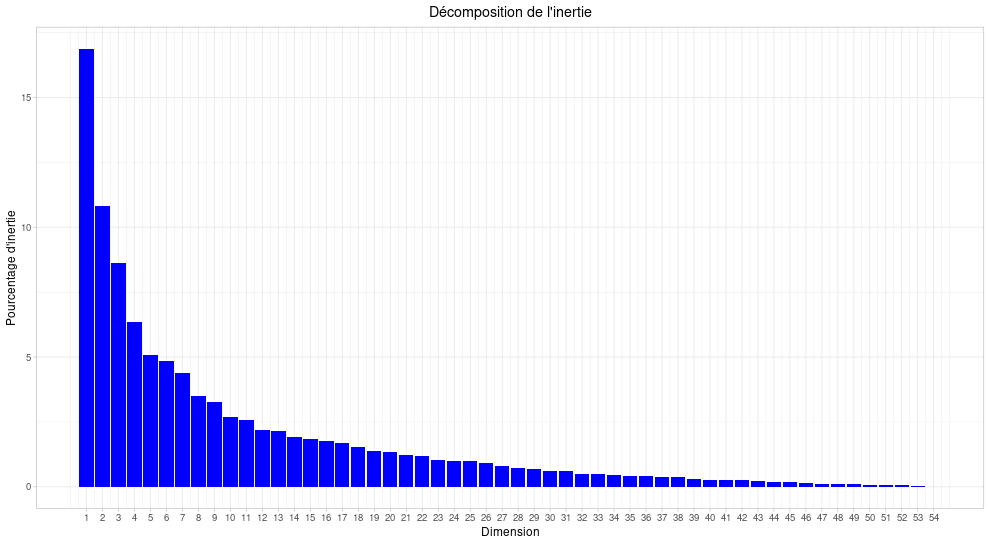
\includegraphics[width=0.8\linewidth]{images/ACPR_vp}}

et le tableau de valeurs :

\begin{center}
 \begin{tabular}{|l|*{8}{>{\centering\arraybackslash}p{1cm}|}}
 \hline 
 \rule[-1ex]{0pt}{2.5ex} Valeurs propres & Dim.1  & Dim.2 &  Dim.3 &  Dim.4 &  Dim.5 &  Dim.6 &  Dim.7 & Dim.8\\ 
 \hline 
 \rule[-1ex]{0pt}{2.5ex}  Variance & 9.110 &   4.511 &  4.662 &  3.422 &  2.752 &  2.616  & 2.358 &  1.879\\
 \hline 
 \rule[-1ex]{0pt}{2.5ex} 
$\%$ of var. &  16.871 & 10.825 &  8.634 &  6.338 &  5.096 &  4.844  & 4.366 &  3.480 \\
 \hline 
 \rule[-1ex]{0pt}{2.5ex} 
Cumulative $\%$ of var. & 16.871 & 27.696 & 36.330 & 42.668 & 47.764 & 52.608 & 56.974 & 60.455 \\
\hline
\end{tabular}
\end{center}

On a un décrochement entre la 4-ème et la 5-ème valeurs ce qui nous pousse à nous intéresser aux quatre premiers axes. C'est déjà une différence avec l'ACP normée. 

\subsection{Etude des différents plans}

{\large \textbf{Plan (1,2)}}

Côte à côte voici les graphiques des individus et celui des variables avec les 25 plus gros contributeurs pour les individus et les 10 plus gros contributeurs pour les variables : 

\centerline{\begin{tabular}{ccc}
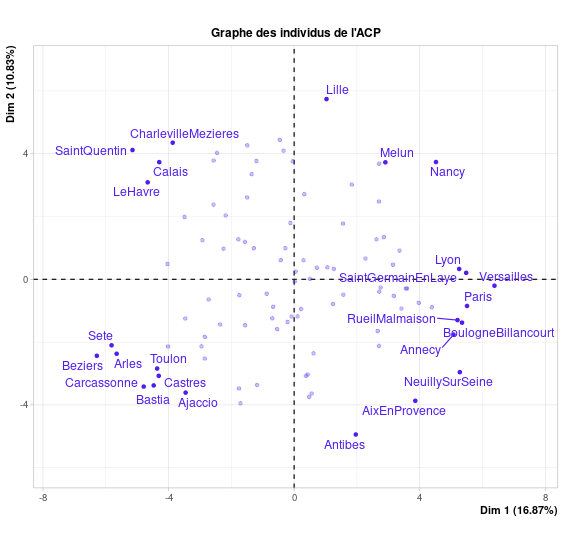
\includegraphics[width=0.55\linewidth]{images/ACPR_ind_12} & 
&
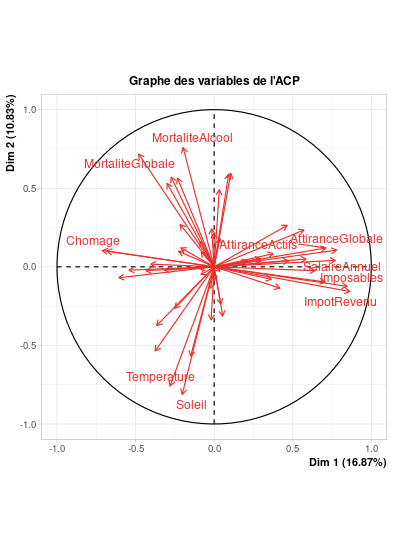
\includegraphics[width=0.40\linewidth]{images/ACPR_var_12}
\end{tabular}}

On retrouve le même faisceau des variables de richesse que sur l'ACP normée, auxquelles viennent se rajouter \emph{AtiranceActifs} et \emph{AttiranceGlobale}. Ces variables sont à mettre en opposition à la variable chômage qui décrit plus la pauvreté. Dans la même direction se trouvent les villes trouvées lors de l'ACP normée, celle de l'Ouest parisien. Des villes réputées riches comme \emph{Lyon}, \emph{Annecy} ou bien \emph{Aix-en-Provence} viennent compléter la liste.


\textbf{Tableau des variables les plus contributrices pour l'axe 1 :}
\begin{center}
\begin{tabular}{|c|c|c|c||c|c|c|c|}
\multicolumn{4}{c}{Côté -} & \multicolumn{4}{c}{Côté +}\\
\hline 
Variables & Coordonnées & CTR & COS2 & COS2 & CTR & Coordonnées & Variables \\ 
\hline 
Chômage & $-0.71$ & $5.55$ & $0.51$ & $0.75$ & $8.19$ & $0.86$ & ImpotRevenu  \\ 
\hline 
 &  &  &  & $0.71$ & $7.85$ & $0.85$ & Imposables\\ 
\hline 
 &  &  &  & $0.61$ & $6.67$ & $0.78$ & AttiranceGlobale \\ 
\hline 
\end{tabular} 
\end{center}

\bigskip

\textbf{Tableau des individus les plus contributeurs pour l'axe 1 :}
\begin{center}
\begin{tabular}{|c|c|c|c||c|c|c|c|}
\multicolumn{4}{c}{Côté -} & \multicolumn{4}{c}{Côté +}\\
\hline 
Villes & Coordonnées & CTR & COS2 & COS2 & CTR & Coordonnées & Villes \\ 
\hline 
Beziers & $-6.28$ & $4.33$ & $0.57$ & $0.58$ & $4.47$ & $6.38$ & Versailles \\ 
\hline 
Sète & $-5.81$  & $3.71$ & 0.41 & $0.44$ & $3.33$ & $5.51$ & Paris\\ 
\hline 
 &  &  &  & $0.40$ & $3.30$ & $5.48$ & Saint-Germain-En-Laye \\ 
\hline 
\end{tabular} 
\end{center}

Sur cet axe 1, il y a plusieurs points contributifs, mais peu sont illustratifs car seuls les COS2 de \emph{ImpotRevenu} et \emph{Imposables} sont importants.

\bigskip

L'axe 2 met en opposition des villes du Sud et du Nord avec deux groupes bien distincts. Ceci correspond à une opposition entre les variables \emph{Température}, \emph{Soleil} et les variables \emph{MortaliteAlcool} et \emph{MortaliteGlobale}. Ceci est clairement visible sur les deux tableaux suivants :

\textbf{Tableau des variables les plus contributrices pour l'axe 2 :}
\begin{center}
\begin{tabular}{|c|c|c|c||c|c|c|c|}
\multicolumn{4}{c}{Côté -} & \multicolumn{4}{c}{Côté +}\\
\hline 
Variables & Coordonnées & CTR & COS2 & COS2 & CTR & Coordonnées & Variables \\ 
\hline 
Soleil & $-0.81$ & $11.27$ & $0.66$  & $0.58$  & $9.85$ & $0.76$ & MortaliteAlcool  \\ 
\hline 
 Temperature& $-0.76$ & $9.83$ & $0.57$ & $0.51$ & $8.80$ &  $0.72$ & MortaliteGlobale\\ 
\hline 
Vieillissement & $-0.57$  & $5.52$ & $0.32$ &  &  & &  \\ 
\hline 
\end{tabular} 
\end{center}

\bigskip

\textbf{Tableau des individus les plus contributeurs pour l'axe 2 :}
\begin{center}
\begin{tabular}{|c|c|c|c||c|c|c|c|}
\multicolumn{4}{c}{Côté -} & \multicolumn{4}{c}{Côté +}\\
\hline 
Villes & Coordonnées & CTR & COS2 & COS2 & CTR & Coordonnées & Villes \\ 
\hline 
Antibes & $-4.94$ & $4.18$ & $0.33$ & $0.52$ & $5.64$ & $5.74$ & Lille \\ 
\hline 
 &   &  &  & $0.33$ & $3.38$ & $4.44$ & Valenciennes\\ 
\hline 
 &  &  &  & $0.22$ & $3.12$ & $4.27$ & Saint-Denis\\ 
\hline 
\end{tabular} 
\end{center}


{\large \textbf{Plan (3,4)}}

\centerline{\begin{tabular}{ccc}
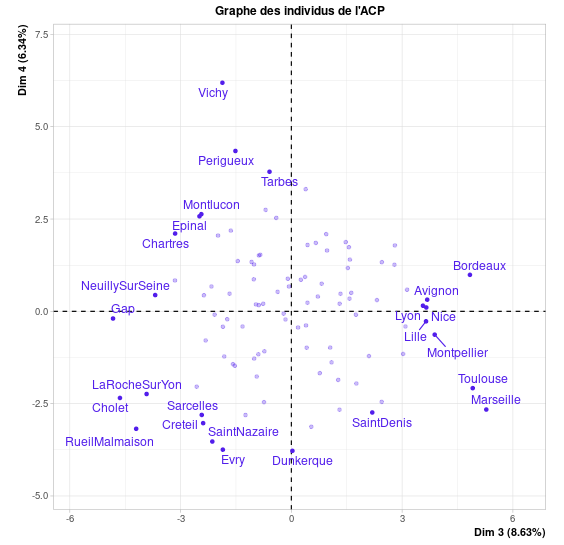
\includegraphics[width=0.55\linewidth]{images/ACPR_ind_34} & 
&
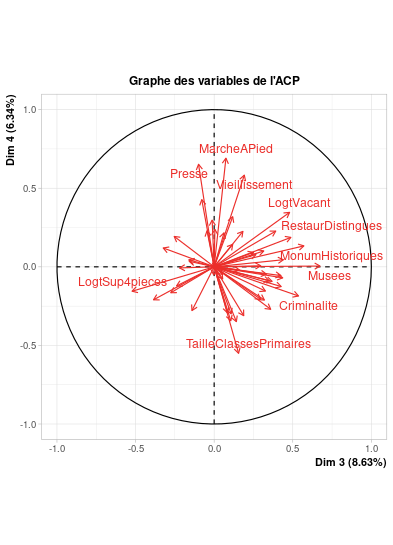
\includegraphics[width=0.40\linewidth]{images/ACPR_var_34}
\end{tabular}}

En observant ces deux graphiques, il ressort que les variables les mieux représentées pour l'axe 3 sur le plan sont \emph{Musées}, \emph{MonumHistoriques}, \emph{Criminalité} et \emph{RestauDistingue}. Ces variables sont corrélées négativement à \emph{LogtSup4Pieces}. En regardant de plus près les individus contributeurs, on trouve des grandes villes françaises à droite qui font la part belle à la culture mais où la criminalité est importante. Par criminalité, il faut entendre le nombre d'infractions et délits commis. Les infractions relatives au code de la route y sont forts nombreuses dans les grandes villes.

\textbf{Tableau des variables les plus contributrices pour l'axe 3 :}
\begin{center}
\begin{tabular}{|c|c|c|c||c|c|c|c|}
\multicolumn{4}{c}{Côté -} & \multicolumn{4}{c}{Côté +}\\
\hline 
Variables & Coordonnées & CTR & COS2 & COS2 & CTR & Coordonnées & Variables \\ 
\hline 
LogtSup4Pieces & $-0.52$ & $5.85$ & $0.27$  & $0.45$  & $9.72$ & $0.67$ & Musées  \\ 
\hline 
&  &  &  & $0.33$ & $6.99$ &  $0.57$ &  MonumHistoriques\\ 
\hline 
&  &  &  & $0.29$ & $6.18$ & $0.54$ & Criminalité \\ 
\hline 
&  &  &  & $0.32$ & $5.11$ & $0.49$ & RestauDistingues \\ 
\hline
\end{tabular} 
\end{center}

\bigskip

\textbf{Tableau des individus les plus contributeurs pour l'axe 3 :}
\begin{center}
\begin{tabular}{|c|c|c|c||c|c|c|c|}
\multicolumn{4}{c}{Côté -} & \multicolumn{4}{c}{Côté +}\\
\hline 
Villes & Coordonnées & CTR & COS2 & COS2 & CTR & Coordonnées & Villes \\ 
\hline 
Gap & $-4.83$ & $5$ & $0.33$ & $0.44$ & $5.98$ & $5.28$ & Marseille\\
\hline
 Cholet & $-4.64$  & $4.62$  & $0.33$ & $0.43$ & $5.17$ & $4.91$ & Toulouse\\ 
\hline 
 &  &  &  & $0.40$ & $5.02$ & $4.84$ & Bordeaux\\ 
\hline 
\end{tabular} 
\end{center}

La principale différence avec l'ACP normée c'est que l'on ne retrouve pas Paris sur cet axe alors qu'il en était le principal contributeur précédemment. Le fait de faire une ACP de rang à éliminer une grande partie de la singularité de Paris et les variables culturelles qui la décrivait. Ici les COS2 sont plutôt faibles et l'originalité des villes est partiellement mis en évidence ici.

\bigskip

Sur l'axe 4, trois variables ont une forte contribution : \emph{MarcheAPied} (13.95), \emph{Presse} (12.43) et \emph{Vieillissement} (9.94). Pour ce qui est des villes, deux sortent du lot \emph{Vichy} (11.20) et \emph{Tarbes} (4.17). L'originalité de Vichy est tirée à 50\% par ces variables et à 31\% pour Tarbes. Concernant les variables, \emph{MarcheaPied} tire 48\% de son originalité le long de cet axe, 43\% pour \emph{Presse} et 34\% pour \emph{Vieillissement}. 

\bigskip

Ces trois variables semblent décrire des variables liées à une population de retraités. Il faudrait regarder plus en détail les villes concernées pour en avoir le c\oe ur net.  

 

   








\section{ACP normé pour les différents thèmes}

\section{ACP de rang pour les différents thèmes}





 
\end{document}
